\documentclass{article}
\usepackage[utf8]{inputenc}

\usepackage{calc}
\usepackage{eso-pic}
\newlength{\PageFrameTopMargin}
\newlength{\PageFrameBottomMargin}
\newlength{\PageFrameLeftMargin}
\newlength{\PageFrameRightMargin}

\setlength{\PageFrameTopMargin}{1cm}
\setlength{\PageFrameBottomMargin}{1cm}
\setlength{\PageFrameLeftMargin}{1cm}
\setlength{\PageFrameRightMargin}{1cm}

\makeatletter

\newlength{\Page@FrameHeight}
\newlength{\Page@FrameWidth}

\AddToShipoutPicture{
   \thinlines
   \setlength{\Page@FrameHeight}{\paperheight-\PageFrameTopMargin-\PageFrameBottomMargin}
   \setlength{\Page@FrameWidth}{\paperwidth-\PageFrameLeftMargin-\PageFrameRightMargin}
   \put(\strip@pt\PageFrameLeftMargin,\strip@pt\PageFrameTopMargin){
   \framebox(\strip@pt\Page@FrameWidth, \strip@pt\Page@FrameHeight){}}}

\makeatother

\usepackage{graphicx}

\title{Testing the document}
\author{Ayyappa Koppuravuri}

\graphicspath{{Images/}}

\begin{document}
\maketitle
\tableofcontents

\newpage
Helmo


\begin{figure}[h]
	\raggedright
	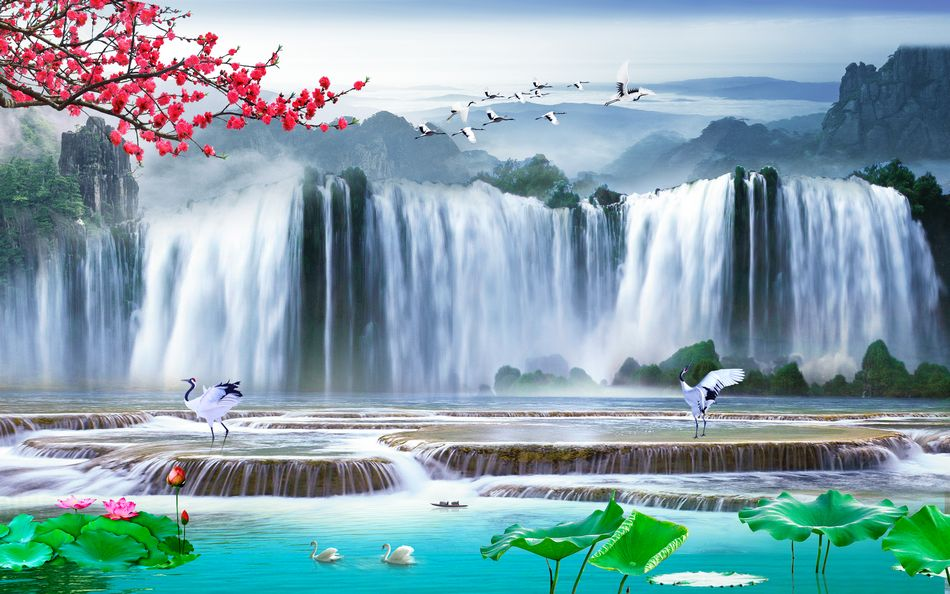
\includegraphics[width=5cm]{image1.jpg}
	\caption{This is a left aligned image}
\end{figure}

\section{Story}
This is the content of the story

\begin{figure}[h]
	\raggedleft
	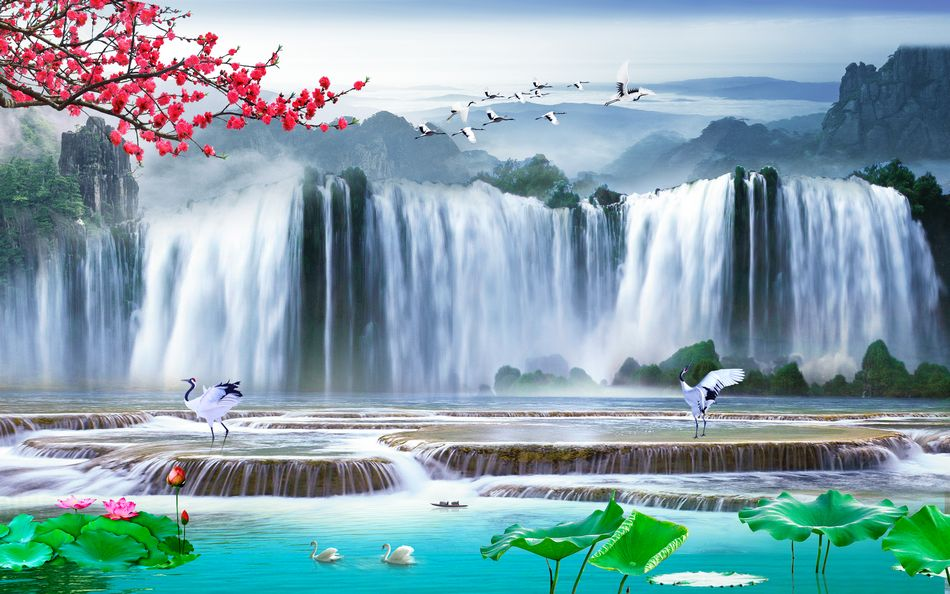
\includegraphics[width=5cm]{image1.jpg}
	\caption{This is a right aligned image}
\end{figure}



\subsection{story part1}
This is the content belonging to part1 of the story

\subsubsection{story part1.1}
This is the content belonging to part1.1 of the story

\section*{Story1}
This is the content of story 1
\newpage


\subsection*{Story1 part1}
This is the content belonging to part1 of the story1

\begin{figure}[h]
	\centering
	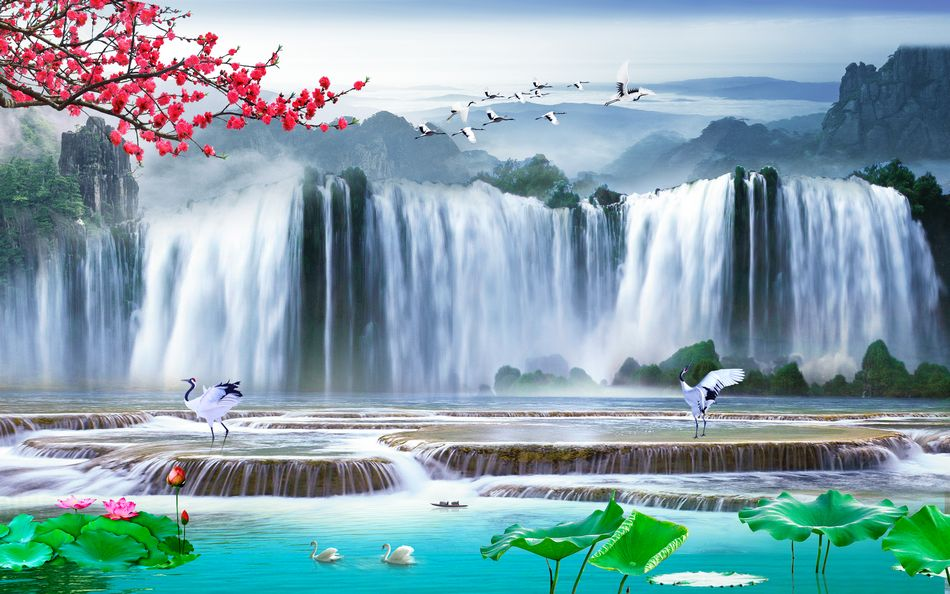
\includegraphics[width=5cm]{image1.jpg}
	\caption{This is a Center aligned image}
\end{figure}



\subsubsection*{Story1 part1.1}
This is the content belonging to part1 of the story1.1

\end{document}
